% \textbf{Title: Vectors 4}

Consider these vectors.

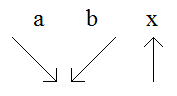
\includegraphics[width=1.84401in,height=1.00014in]{../../Images/VectorsQ4.png}

The vectors are all to scale. How can we express \(\overrightarrow{x}\) in terms of \(\overrightarrow{a}\) and \(\overrightarrow{b}\)? \\

a. \(\overrightarrow{x} = \overrightarrow{a} + \overrightarrow{b}\)

b. \(\overrightarrow{x} = - \left( \overrightarrow{a} + \overrightarrow{b} \right)\)

c. \(\overrightarrow{x} = \frac{1}{2}\left( \overrightarrow{a} + \overrightarrow{b} \right)\)

*d. \(\overrightarrow{x} = - \frac{1}{2}\left( \overrightarrow{a} + \overrightarrow{b} \right)\)

e. I do not know. \\
